%!TEX root = ../report.tex
\chapter{Experiment Setup}
In this chapter the experimental setup is outlined. For the experiment, a number of simulation runs are performed in USAR Sim, which are recorded. We will encounter a number of cases where the ManifoldSLAM scan matcher fails. 

\section{Map Stitching}
Map stitching prior work, magda etc

\section{SLAM confidence measure}
The confidence measure based on the determinant of the covariance matrix of the pose uncertainty. The hypothesis is that if this measure is larger, then the confidence is lower (the uncertainty is bigger).

The determinant of the covariance matrix is used as metric:

is the sample variance-covariance matrix for observations of a multivariate vector of p elements. The determinant of D, in this case, is sometimes called the generalized variance. (http://www.itl.nist.gov/div898/handbook/pmc/section5/pmc532.htm)

\section{Inertial sensor data}
Gives the rotations on three axis, enables you to detect 

\section{Confidence measures}
cite bayu and max:     Good examples of single confi- dence values that can be derived from a covariance matrix are the determinant det(Σ) or the trace trace(Σ). The relations lend themselves very well for use in path-planning and search algorithms. In addition, heuristic algorithms can take advantage of the uncertainty information stored on the links. (P61)


%http://areeweb.polito.it/ricerca/MacP4Log/images/poster_SIDRA2009.pdf
(paper not found): L. Carlone, M. Kaouk Ng, J. Du, B. Bona, and M. Indri, “Reverse KLD-Sampling for measuring uncertainty in Rao-Blackwellized Particle Filters SLAM”, in Proc. of the 2009 IEEE/RSJ Int. Conf. on Intelligent RObots and Systems, Workshop on Performance Evaluation and Benchmarking for Next Intelligent Robots and Systems, 2009.

Carlone et al. use a particle filter based representation of their belief. 

\begin{figure}[ht]
  \begin{center}
    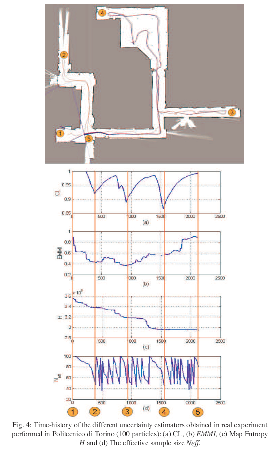
\includegraphics[scale=2]{images/poster_SIDRA2009_result.pdf}
  \end{center}
  \caption{}
  \label{fig:carlone}
\end{figure}

In this work we examine a few different confidence measures:
1) attack angle
2) determinant of match
3) trace of match

From SlametPfingstorn:

To asses the quality of fit
of a new range scan, the same notion of being well-fitted is used as during the construction
of local sub-maps (refer to Section 5.3.3). Recall that we already obtained the covariance
matrix Σt of the Gaussian distribution that was estimated by the scan matcher. The Fisher
information matrix I is computed by taking the inverse of this covariance matrix I = Σ−1 ttt
and we compute the 95% confidence interval for every pose variable as follows: σ = 1.96􏰌􏰀I−1􏰁